%
%
%
% ESTA SECCION SE ENCUENTRA LEÍDA, CORREGIDA Y "CERRADA".
% PARA EVITAR INCONVENIENTES, POR FAVOR, 
% NO MODIFICAR A ULTIMO MOMENTO SIN AVISAR AL RESTO DEL GRUPO.
%
%
%
% ------ headers globales y begin ---------------
\documentclass[11pt, a4paper, twoside]{article}
\usepackage{header_tp2}
\begin{document}{}
% -----------------------------------------------
Se tiene un campo cuadrado de $n \times n$ celdas, cada una de la cuales tiene un resorte propulsor con 
una potencia que va de 1 a $p$. Es decir que es posible ir saltando de una celda cualquier otra mediante estos 
resortes. El juego consiste en que cada participante llegue a la celda $destino$ partiendo 
desde la celda $origen$, realizando la menor cantidad de saltos posibles. Para moverse de una de una celda a otra, 
sólo se permiten movimientos hacia el norte, sur, este u oeste. La potencia que tenga el resorte en una celda, 
es la que limitará la distancia del salto que se puede realizar desde una celda a otra. Además, el participante 
contará con una cantidad $k$ de pontencia extra, la cual podrá utilizar durante el juego, distribuyéndola como le 
sea conveniente en cada salto. Esta potencia extra, le permitirá realizar saltos de mayor distancia. 
La complejidad temporal de peor caso del algoritmo deberá ser de $\bigO{{n^3} \times k}$. \\

\centerbf{Formato de entrada y salida:} 

	\begin{center}
		\begin{minipage}{0.5\textwidth}
			\begin{tabular}{cccccc}
			   & Input \\
			   \hline 
			   n        & $f_{0}$  & $c_{0}$   & $f_{d}$ & $c_{d}$ & k \\
			   $p_{11}$ & $\hdots$ & $p_{1n}$  &&& \\
			   $\vdots$ &          &  $\vdots$ &&& \\
			   $p_{n1}$ &        &  $p_{nn}$   &&& \\
			\end{tabular}
		\end{minipage} 
		\begin{minipage}{0.1\textwidth}
			\begin{tabular}{ccc}
					& Output \\
				   \hline
				   S &   &   \\
				   $f_1$ & $c_1$ & $e_1$ \\
				   $\vdots$ & $\vdots$& $\vdots$\\
				   $f_s$ & $c_s$ & $e_s$ \\
			\end{tabular}
		\end{minipage} 	
	 \end{center} 
	
	\begin{itemize}
		\item n $\#filas$ y $\#columnas$
		\item $(f_{0},c_{0})$ celda $origen$
		\item $(f_{d},c_{d})$ celda $destino$
		\item k $\#unidades$ de potencia extra
		\item $p_{ij}$ potencia máxima del resorte de la celda (i,j), $1 < i,j < n$
		\item S $\#saltos$ de solución óptima
		\item $(f_{i},c_{i})$ celda a la que se realiza el salto, $1 < i < S$
		\item ${e_i}$ $\#unidades$ de potencia extra usados en saldo $i$, $1 < i <S$, $0 < e_i < k$	\\
	\end{itemize} 
 

\begin{samepage}

\begin{ejemplo}\hspace{0em} \\
    \begin{center}
	\begin{minipage}{0.4\textwidth}
			\begin{tabular}{cccccc}
			 & Input \\
			   \hline
			   3 & 1 & 1 & 2 & 3 & 2\\
			   1 & 1 & 1 &   &   &  \\
			   1 & 2 & 1 &   &   &  \\
			   1 & 1 & 1 &   &   &  \\
			\end{tabular}
	\end{minipage}
	\end{center}
	
La siguientes son algunas soluciones posibles (las 2 primeras serían las óptimas): \\	

 \begin{center}
	\begin{minipage}{0.3\textwidth}
			\begin{tabular}{ccc}
				   & Output\\
				   \hline
				   2 &   &   \\
				   2 & 1 & 0 \\
				   2 & 3 & 1 \\
				   \\
				   \\
			\end{tabular}
	\end{minipage} 	
	\begin{minipage}{0.3\textwidth}
			\begin{tabular}{ccc}
				   & Output\\
				   \hline
				   2 &   &   \\
				   1 & 3 & 1 \\
				   2 & 3 & 0 \\
				   \\
				   \\
			\end{tabular}
	\end{minipage} 	\\
	\begin{minipage}{0.3\textwidth}
			\begin{tabular}{ccc}
				   & Output\\
				   \hline
				   3 &   &   \\
				   1 & 2 & 0 \\
				   1 & 3 & 0 \\
				   2 & 3 & 0 \\
				   \\
			\end{tabular}
	\end{minipage} 	
	\begin{minipage}{0.3\textwidth}
			\begin{tabular}{ccc}
				   & Output\\
				   \hline
				   3 &   &   \\
				   3 & 1 & 1 \\
				   3 & 3 & 1 \\
				   2 & 3 & 0 \\
				   \\
			\end{tabular}
	\end{minipage} 	
	\begin{minipage}{0.3\textwidth}
			\begin{tabular}{ccc}
				   & Output\\
				   \hline
				   4 &   &   \\
				   2 & 1 & 0 \\
				   3 & 1 & 0 \\
				   3 & 3 & 1 \\
				   2 & 3 & 0 \\
			\end{tabular}
	\end{minipage} 	
\end{center}	

\end{ejemplo}
 
\end{samepage}

\begin{figure}[b]
\centering
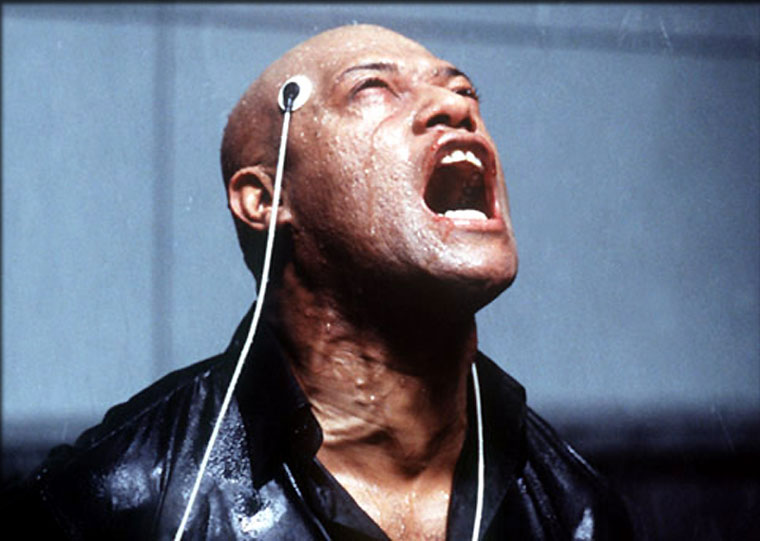
\includegraphics[width=0.5\textwidth]{morfeo.jpg}
\caption{Moerfo, antes de saltar {\footnotesize(...a la siguiente celda)}}
\end{figure}

\end{document}